
\section{Introduction}

\begin{frame}
	\frametitle{Research Area}
	\begin{columns}
		\begin{column}{0.4\textwidth}\centering
		\begin{itemize}
			\item Unmanned Aerial Vehicles (UAVs)
			\item Attitude $(\phi, \theta, \psi)$ and Position $(x, y, z)$ control
			\item Mathematical model embedded with a manifold structure
			\item Two frameworks considered:
			
			\begin{itemize}
				\item Geometric Mechanics and Control
				\item Passive Decomposition
			\end{itemize}
		\end{itemize}
		\end{column}
	
		\begin{column}{0.6\textwidth}\centering
			\begin{figure}[H]
				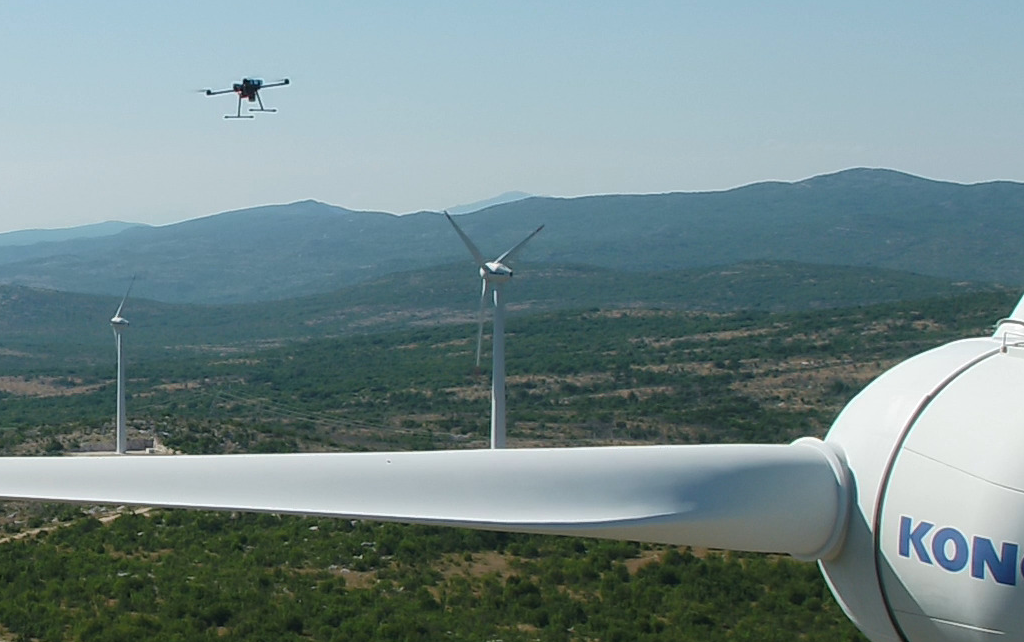
\includegraphics[width=0.9\columnwidth]{figures/drone_flight3_1.png}
				\caption{UAV equipped with a Velodyne LiDAR while performing a wind-turbine inspection.}
			\end{figure}
		\end{column}	
	\end{columns}
\end{frame}

\begin{frame}
	\frametitle{Why Manifolds? (1)}
	\begin{columns}
		
		\begin{column}{0.4\textwidth}\centering
			\begin{figure}[H]
				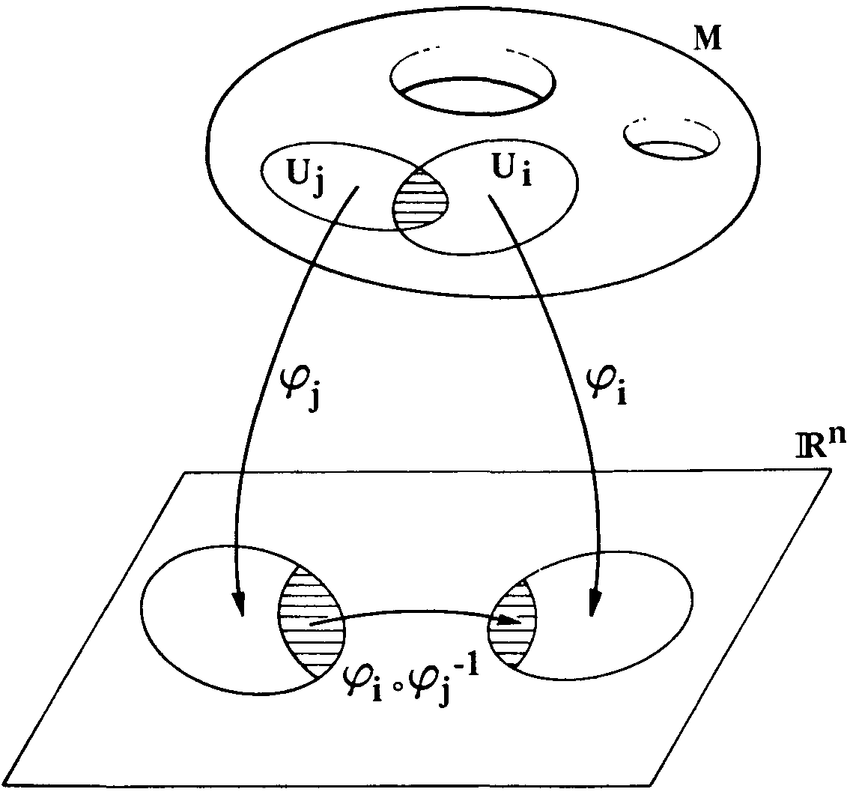
\includegraphics[width=0.9\columnwidth]{figures/manifold.png}	
				\centering
				\caption{Manifold $\Ma$, Euclidean space $\mathbb{R}^n$ and transport maps $\varphi$.\footnotemark}
				\label{fig:aerial_manip}
			\end{figure}
		\end{column}
	
	\begin{column}{0.6\textwidth}\centering
		\begin{itemize}
			\item UAV configuration space:
		\end{itemize}
		\begin{equation}
			\zeta = [x, y, z, \phi, \theta, \psi] 
			\xleftrightarrow{\varphi}
			\text{T} = \begin{bmatrix}
			\text{R} & \textbf{p} \\
			\textbf{0} & 1
			\end{bmatrix}
		\end{equation}
		\begin{equation}
			\zeta \in \mathbb{R}^6  \, , \; \text{T} \in \text{SE(3)} \, , \; \text{R} \in \text{SO(3)}
		\end{equation}
		
		\begin{itemize}
			\item Lie Group
			\begin{itemize}
				\item set of smooth differentiable manifolds
				\item group multiplication and inversion properties
				\item e.g. SO(3), SE(3), $\text{S}^2$
			\end{itemize}
		\end{itemize}
	\end{column}
	\footnotetext[1]{Vladim Belov, "On Geometry and Symmetries in Classical and Quantum Theories of Gauge Gravity"}
	\end{columns}
\end{frame}

\begin{frame}
	\frametitle{Why manifolds? (2)}
	
	\begin{itemize}
		\item Compact model dynamics represented as a Lagrangian / Hamiltonian system
		\item Coordinate-free approach
		\item No singularities
		\item No ambiguities
	\end{itemize}
\end{frame}